\documentclass{article}

\usepackage{mathtools,amsfonts,amssymb}
\usepackage{enumerate}
\usepackage{fullpage}
\usepackage{fancyvrb}
\usepackage{hyperref}
\usepackage{tikz} 

\begin{document}
\thispagestyle{empty}

\begin{center}
  \textbf{\Large Intermediate Test 5}
  \\ \vspace{1em}
  \textbf{\large January Camp 2021}
  \\ \vspace{1em}
  \textbf{\large Time: $4$ hours}
\end{center}

\vspace{12pt}

\begin{enumerate}[1.]

\item % Tim
{\itshape In the acute-angled triangle $ABC$, the foot of the perpendicular from $B$ to $CA$ is $E$. Let $l$ be the tangent to the circumcircle of $\triangle ABC$ at $B$. The foot of the perpendicular from $C$ to $l$ is $F$. Prove that $EF$ is parallel to $AB$.}

We notice that $\angle CEB + \angle CFB = 90^\circ + 90^\circ = 180^\circ$, which implies $CEBF$ is cyclic. We have $\angle CAB = \angle CBF$ by tan-cord theorem, and $\angle CBF = \angle CEF$ by $CEBF$ cyclic. This gives $\angle CAB = \angle CEF$, so $EF||AB$ by corresponding angles.

\item % Russian, probably. Put in by Taariq
{\itshape Let $x$ and $y$ be distinct real numbers such that $$x + 4 = (y - 2)^2 \qquad\text{and}\qquad y + 4 = (x - 2)^2.$$
Find $x^2 + y^2$.}

We take a difference of squares.
\begin{align*}
(x - 2)^2 - (y - 2)^2 &= (y + 4) - (x + 4)\\
(x - y)(x + y - 4) &= y - x\\
(x + y - 4) &= -1\\
x + y &= 3\\
\end{align*}
From line 2 to line 3, we can divide by $(x - y)$ because $x - y \neq 0$ by the fact that $x$ and $y$ are distinct.

Notice our starting equations can be turned into $$y^2 = x + 4y \quad \text{and}\quad x^2 = 4x + y$$ Adding those equations together we get
\begin{align*}
x^2 + y^2 &= 5x + 5y\\
&= 5(x + y)\\
&=15
\end{align*}

\item % Tim
{\itshape There is a group of 6 people that are very suspicious of each other. It is very important to these people which of the rest of the group consider them to be friends. Now, because of the nature of this group, friendship is not a two way street! Person A may consider himself friends with Person B while Person B does not consider the same about Person A. A true friendship is a pair of people who both consider each other to be friends. If we are told that each of these 6 people considers exactly 3 others to be their friend, what is the minimum and maximum number of true friendships that can exist among these 6 people?}

We deal with the maximum case first. Each person has exactly 3 other friends. This means each person can be a part of at most 3 true friendships. We have 6 people total, and since it takes 2 people to have a true frienship, we can have at most $\frac{6\cdot3}{2} = 9$ true friendships. The graph(Figure 1) gives a construction with 9 true friendships. Each node is a person, and a outgoing edge from $A$ to $B$ says that $A$ is a friends with $B$.

\begin{figure}[h]
\centering
\caption{Maximum case}
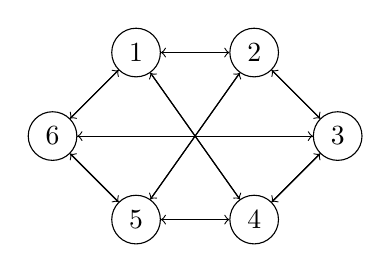
\begin{tikzpicture}[node distance={15mm}, main/.style = {draw, circle}]
\node[main] (1) {$1$};
\node[main] (2) [right of=1] {$2$}; 
\node[main] (3) [below right of=2]{$3$}; 
\node[main] (4) [below left of=3]{$4$}; 
\node[main] (5) [left of =4]{$5$}; 
\node[main] (6) [above left of=5]{$6$}; 
\draw[->] (1) -- (2);
\draw[->] (2) -- (3);
\draw[->] (3) -- (4);
\draw[->] (4) -- (5);
\draw[->] (5) -- (6);
\draw[->] (6) -- (1);
\draw[->] (1) -- (6);
\draw[->] (2) -- (1);
\draw[->] (3) -- (2);
\draw[->] (4) -- (3);
\draw[->] (5) -- (4);
\draw[->] (6) -- (5);
\draw[->] (1) -- (4);
\draw[->] (4) -- (1);
\draw[->] (2) -- (5);
\draw[->] (5) -- (2);
\draw[->] (6) -- (3);
\draw[->] (3) -- (6);
\end{tikzpicture}
\end{figure} 
Now, we deal with the minimum case. We will show that the minimum amount of true friendships is 3 using pigeon hole principle. Notice there are ${6 \choose 2} = \frac{6\cdot5}{2} = 15$ pairs of people. We can consider these 15 pairs to be our pigeon holes by considering the following. Person $A$ being friends with person $B$ is represented by a pigeon being in the pigeon hole for the pair $AB$. Simirlarly, if person $B$ is friends with person $A$ there is an additional pigeon in the pigeon hole $AB$(the same pigeon hole as before). Clearly, a true frienship is when a pigeon hole has 2 pigeons inside. Notice, each of the 6 people have 3 friends, so we have $6\cdot 3 = 18$ pigeons. Each pigeon hole can only take at most 2 pigeons, so by the pigeon hole principle, since we have 18 pigeons and 15 pigeon holes, at least 3 of the pigeon holes must contain 2 pigeons. This means there are at least 3 true friendships. Figure 2 provides a construction that has only 3 true friendships. The construction may seem confusing but in essence person $x$ is connected to person $x + 1$, $x + 2$ and $x + 3$, taking it mod 6 for overflow. The true friendships are between $(1, 4), (2, 5)$ and $(3, 6)$.
\begin{figure}[h]
\centering
\caption{Minimum case}
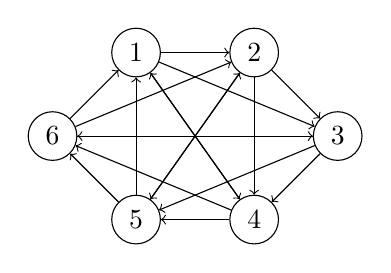
\begin{tikzpicture}[node distance={15mm}, main/.style = {draw, circle}]
\node[main] (1) {$1$};
\node[main] (2) [right of=1] {$2$}; 
\node[main] (3) [below right of=2]{$3$}; 
\node[main] (4) [below left of=3]{$4$}; 
\node[main] (5) [left of =4]{$5$}; 
\node[main] (6) [above left of=5]{$6$}; 
\draw[->] (1) -- (2);
\draw[->] (2) -- (3);
\draw[->] (3) -- (4);
\draw[->] (4) -- (5);
\draw[->] (5) -- (6);
\draw[->] (6) -- (1);
\draw[->] (1) -- (3);
\draw[->] (2) -- (4);
\draw[->] (3) -- (5);
\draw[->] (4) -- (6);
\draw[->] (5) -- (1);
\draw[->] (6) -- (2);
\draw[->] (1) -- (4);
\draw[->] (2) -- (5);
\draw[->] (3) -- (6);
\draw[->] (4) -- (1);
\draw[->] (5) -- (2);
\draw[->] (6) -- (3);
\end{tikzpicture}
\end{figure} 

\item % Ireland 2017 Q7
{\itshape Consider relatively prime integers $a$ and $b$ and a prime number $p$.
Show that
\[ \gcd(ab, a^2+pb^2) = \begin{cases*} 1 & if $p \nmid a$ \\ p & if $p \mid a$ \end{cases*}. \]}

Case 1: $p \nmid a$ \par
We will assume for contradiction that $\gcd(ab, a^2+pb^2) > 1$. Let $d = \gcd(ab, a^2+pb^2)$ and let $q$ be any prime divisor of $d$. 
Then we have that $d \mid ab$ and $d \mid a^2+pb^2 \implies q \mid ab$ and $q \mid a^2+pb^2$. Since $q \mid ab$ and $a$ and $b$ are relatively prime, we have that either $q \mid a$ or $q \mid b$. \par
If $q \mid a$: since we had $q \mid a^2 + pb^2 \implies q \mid pb^2 \implies q \mid p$ or $q \mid b$. The first case would mean that $q = p$ since both are prime and thus that $p \mid a$ which would be a contradiction and the second would contradict the condition that $a$ and $b$ cannot both be divisible by $q$. \par
If $q \mid b$: $q \mid a^2 + pb^2 \implies q \mid a^2 \implies q \mid a$ which is a contradiction since we assumed only one of $a$ or $b$ is divisible by $q$. \par
In conclusion, we have that $\gcd(ab, a^2+pb^2) > 1$ is not true and thus $\gcd(ab, a^2+pb^2) = 1.$ \newline

Case 2: $p \mid a$ \par
Let $a = pk$ where $k$ is a natural number. Note that since $\gcd(a, b) = 1$ we will also have $\gcd(k, b) = 1$ and $\gcd(p, b) = 1.$ \par
We can then say $\gcd(ab, a^2+pb^2) = \gcd(pkb, p^2k^2 + pb^2) = p\cdot \gcd(kb, pk^2 + b^2).$ Assume for contradiction that $\gcd(kb, pk^2 + b^2) > 1$. Let $d = \gcd(kb, pk^2 + b^2)$ and let $q$ be any prime divisor of $d$. Then either $q \mid k$ or $q \mid b$. \par
If $q \mid k$: since we had $q \mid pk^2 + b^2 \implies q \mid b^2 \implies q \mid b$. However, this would be a contradiction since we assumed that $k$ and $b$ cannot both be divisible by $q$. \par
If $q \mid b$ we will have  $q \mid pk^2 + b^2 \implies q \mid pk^2 \implies q \mid p$ or $q \mid k$ . However, since we had that $\gcd(k, b) = 1$ and $\gcd(p, b) = 1$, we cannot have $k$ or $p$ divisible by $q$ as this would mean that $\gcd(k, b) > 1$ or $\gcd(p, b) > 1$. \par
In conclusion we will have that $\gcd(kb, pk^2 + b^2) = 1 \implies \gcd(ab, a^2+pb^2) = p\cdot 1 = p$.


\item % Tim
{\itshape A square-based pyramid has all of its edges the same length.
A cube is placed inside so that one of its faces lies on the base of the pyramid, and the opposite face has an edge along each side of the pyramid (think -- the natural way to put a cube in a pyramid).
Show that the sum of any of the cube's edge lengths with any of the cube's face diagonal lengths is the same as the edge length of the pyramid.}

Let the base of the square pyramid consist of the square $ABCD$, and the top of the pyramid be point $T$.
Consider the plane $P$ through points $A$, $T$, and $C$; by the way the cube is placed inside the pyramid, this plane passes through four points of the cube, the intersection of the plane with the surface of the cube being diagonals of the upper and lower faces and two opposite edges; let these edges be $WX$ and $YZ$ respectively.
Finally, let the edge lengths of the cube and pyramid be $a$ and $b$ respectively; by Pythagoras, $XY = \sqrt{2} YZ = \sqrt{2} a$ and $AC = \sqrt{2} AT = \sqrt{2} b$.
Considering the intersection of the plane $P$ with the pyramid and the cube, we have a rectangle with $\sqrt{2}$ the ratio of width to height inside an isosceles triangle with a right angle at the top.

We place this on the Cartesian plane centred at the midpoint of the base of the triangle, with the top at $(0,b/\sqrt{2})$ and the other two vertices at $(\pm b/\sqrt{2},0)$; then the vertices of the rectangle are at $(\pm a/\sqrt{2},0)$ and $(\pm a/\sqrt{2},a)$.
The equation of the side of the triangle on the right is $y = b/\sqrt{2} -x$; since the point $(\pm a/\sqrt{2},a)$ of the rectangle lies on this side, we have
\[ a = b/\sqrt{2} -a/\sqrt{2} \iff b = \sqrt{2} a + a \]
as desired.


\item % Ireland 2017 Q15
{\itshape There is a soccer competition with five teams where each team plays exactly one match against each other team.
If one team wins against another team, that team gets $5$ points whereas the losing team gets $0$ points.
If two teams draw, they each get $1$ point if neither team scored a goal and they each get $2$ points if they scored at least one goal.
At the end of the competition it is found that the total points for the teams form five consecutive nonnegative integers.
What is the minimum number of goals scored in this competition?}


\textbf{Solution 1}\\
Ten matches are played each one contributing either 2, 4 or 5 points. Hence the total number of points is between 20 and 50. If the team scores are five consecutive integers, then the total number of points must be a multiple of 5. If the total number of points is 20, all teams will score 4 and if the total number of points is 50 all team totals will be multiples of 5. Neither of these possibilities satisfy the conditions. Therefore, we need to consider the following five cases:
\begin{itemize}
	\item [(a)] scores are 3, 4, 5, 6, 7,
	\item [(b)] scores are 4, 5, 6, 7, 8,
	\item [(c)] scores are 5, 6, 7, 8, 9,
	\item [(d)] scores are 6, 7, 8, 9, 10 and
	\item [(e)] scores are 7, 8, 9, 10, 11.
\end{itemize}
Case (a): Number of wins is odd. 3 wins yield 15 points and the other seven matches yield more than 10 points. The only possibility is one win, 8 0-0 draws and one score draw. But the team that wins must gain at least 3 points in the other matches. Hence this case is impossible.\\
Case (b): The number of wins is even and cannot be 4 as only three teams have a score of five or more and none have a score of 10. No wins means there are 5 score draws and 5 no score draws. The teams scoring 8 and 7 must be involved in 7 score draws to achieve these totals. Hence, the only possibility is 2 wins 2 score draws and 6 no score draws. The table

\begin{table}[ht!]
	\begin{center}
	  \begin{tabular}{ | c | c | c | c | c | c | c |}
		  \hline
		    & A & B & C & D & E & Total\\
		  \hline  
		  A &   & 5 & 1 & 1 & 1 & 8\\
		  \hline  
		  B & 0 &   & 1 & 1 & 5 & 7\\
		  \hline  
		  C & 1 & 1 &   & 2 & 2 & 6\\
		  \hline  
		  D & 1 & 1 & 2 &   & 1 & 5\\
		  \hline  
		  E & 1 & 0 & 2 & 1 &   & 4\\
		  \hline  
	  \end{tabular}
	\end{center}
\end{table}

realizes this possibility. The minimum number of goals in this case is 6.\\
Case (c): The number of wins is odd. No team has more than one win. If the number of wins is five, each team must win one match and all other matches are no score draws. A total of 9 is now impossible. If the number of wins is 3, there most be 3 score draws and 4 no score draws. At least 9 goals are scored in this scenario. If the number of wins is 1, there are 6 score draws and three no score draws. This gives at least 13 goals.\\
Case (d): Again we can calculate the number of wins $(W)$, score draws $(S)$ and no score draws $(N)$ yielding 40 points. The four possibilities are $(W, S, N) = (6, 1 3)$ or (4, 4, 2) or (2, 7, 1) or (0, 10, 0). The minimum number of goals is $W + 2S$ which in each case is bigger than 6.\\
Case (e): Calculating possible values of $(W, S, N)$ we obtain (7, 2, 1), (5, 5, 0) giving more than 6 goals.
Thus the minimum number of goals scored in the tournament is 6.\\
\newline
\textbf{Solution 2}
If the five consecutive scores of the teams are $a-2, a-1, a, a+1, a+2$, the total number of points is $5a$. Each match contributes 5, 4 or 2 points to this total.\\
Let $w$ be the number of matches that did not end in a draw, $d_0$ the number of 0-0 draws and $d_1$ the number of draws with goals. The minimal possible number of goals scored is $g = w + 2d_1$. The number of matches is ${5 \choose 2} = 10$, so we obtain
\begin{eqnarray*}
w + d_0 + d_1 & = & 10\\
5w + 2d_0 + 4d_1 & = & 5a.
\end{eqnarray*}
Eliminating $d_0$ from these equations we obtain $3w + 2d_1 = 5(a-4)$. This equation implies $3w = -2d_1$ (mod 5), hence $w = d_1$ (mod 5).\\
None of $w$, $d_1$ and $w+d_1$ can exceed 10. Hence, $d_1 = w + 5t$ with $-2 \leq t \leq 2$. We obtain $g = w + 2d_1 = 3w + 10t$.
\begin{itemize}
\item  If $t = -2$, we have $w = d_1 + 10 \leq 10$, hence $w = 10$, $d_1 = 0$ and $g = 10$.
\item  If $t = -1$, we have $d_1 = w - 5 \geq 0$ and $w + d_1 = 2w - 5 \leq 10$, hence $5 \leq w + 7$. If $w \geq 6$, we have $g = 3w - 10 \geq 8$. For $w = 5$, we get $g = 5$.
\item  If $t = 0$,  and $w \geq 3$ we have $g = 3w + 10t \geq 9$.
\item  If $t \geq 1$, we have $g \geq 10$.
\end{itemize}
Hence, there are only four cases in which $g \leq 6$. They are all shown in the table below. The values of $d_0$, $a$ and $g$ are obtained from the equations above.

\begin{table}[ht!]
	\begin{center}
	  \begin{tabular}{ | c | c | c | c | c | c |}
		  \hline
		  Case &  $w$ & $d_1$ & $d_0$ & $a$ & $g$ \\
		  \hline  
		  1 & 0 & 0 & 10 & 4 & 0 \\
		  \hline  
		  2 & 1 & 1 &  8 & 5 & 3 \\
		  \hline  
		  3 & 5 & 0 &  5 & 7 & 5 \\
		  \hline
		  4 & 2 & 2 &  6 & 6 & 6\\
		  \hline  
	  \end{tabular}
	\end{center}
\end{table}

Case 1: If $d_0 = 10$ all matches were no score draws, hence all teams scored 5 points contradicting the conditions.\\
Case 2: If $a = 5$, the winning team achieved 7 points. But, if $w = 1$ the team who has one one match cannot have lost any of their matches, hence would have scored at least 8 points.\\
Case 3: If $a = 7$, the maximum number of points a team scored is 9, hence no team won two matches. As $d_1 = 0$, the top team can have scored at most 3 points from the matches it didn't win, hence cannot have got 9 points in total.\\
Case 4: This case is actually possible, as the following table shows.
\begin{table}[ht!]
	\begin{center}
	  \begin{tabular}{ | c | c | c | c | c | c | c |}
		  \hline
		    & A & B & C & D & E & Total\\
		  \hline  
		  A &   & 5 & 1 & 1 & 1 & 8\\
		  \hline  
		  B & 0 &   & 1 & 1 & 5 & 7\\
		  \hline  
		  C & 1 & 1 &   & 2 & 2 & 6\\
		  \hline  
		  D & 1 & 1 & 2 &   & 1 & 5\\
		  \hline  
		  E & 1 & 0 & 2 & 1 &   & 4\\
		  \hline  
	  \end{tabular}
	\end{center}
\end{table}

Therefore, the minimum number of goals scored is 6.

\end{enumerate}


\clearpage
~
\vfill
% ASCII art
\centering
% \tiny
The duck in this paper was an affront to God, and so has been removed.
\vfill

\end{document}
